\chapter{引言与数学基础}

\intro{控制理论研究动态系统的建模、分析与设计方法。本章介绍自动控制理论的发展历程、核心思想与必要的数学预备知识。}

\section{控制理论概述}

\subsection{控制理论的发展简史}

自动控制的起源可追溯至古代文明。公元前3世纪，希腊人Ktesibios发明的水钟利用浮子调节水位实现流量控制，是最早的反馈机构之一。然而，控制理论作为一门系统科学，其发展脉络主要集中在近现代：

\begin{itemize}
\item 工业革命时期（18--19世纪）。James Watt于1788年设计的离心式调速器是自动控制领域的里程碑。该装置利用飞球离心力调节蒸汽机进气阀门，构成速度反馈回路。然而，调速器在特定工况下出现的剧烈振荡——即所谓"猎振"（hunting）现象——引起了J. C. Maxwell的注意。1868年，Maxwell发表了《On Governors》一文，首次从微分方程角度分析了调速系统的稳定性，开创了控制理论的数学化研究。
\item 经典控制时期（1930--1960）。20世纪30年代，Bell实验室的H. Nyquist提出了基于频率响应的稳定性判据，H. W. Bode发展了相应的对数频率特性图（Bode图）。二战期间，火炮伺服系统、雷达跟踪系统等军事需求极大地推动了控制理论的发展。N. Wiener于1948年出版的《控制论》（\emph{Cybernetics}）将反馈概念推广至通信、生物和社会系统。
\item 现代控制时期（1960至今）。1960年，R. E. Kalman提出了状态空间方法和著名的Kalman滤波器，将控制理论从频域的传递函数方法扩展到时域的状态空间框架。此后，最优控制（Pontryagin极大值原理、Bellman动态规划）、鲁棒控制（$H_{\infty}$理论）、自适应控制、非线性控制和非线性观测器等方向蓬勃发展。
\end{itemize}

\subsection{开环控制与闭环控制}

\begin{mydefinition}{开环控制系统}
开环控制系统是指控制器的输出仅取决于参考输入信号，而不依赖于系统实际输出信号的系统。其通用结构为：
\[
\text{参考输入} \rightarrow \text{控制器} \rightarrow \text{执行器} \rightarrow \text{被控对象} \rightarrow \text{输出}
\]
\end{mydefinition}

\begin{mydefinition}{闭环控制系统（反馈控制系统）}
闭环控制系统将系统输出量通过测量元件反馈至输入端，与参考输入比较形成偏差信号，控制器根据偏差产生控制作用。其核心在于"检测偏差，纠正偏差"。
\end{mydefinition}

\begin{example}
以室内温度控制为例：开环方式是根据经验设定加热功率，不检测室温；闭环方式则通过温度传感器实时测量室温，与设定温度比较后自动调节加热功率。若门窗意外开启，开环系统无法补偿热量散失，而闭环系统能自动增大加热功率以维持设定温度。
\end{example}

\begin{remark}
反馈的引入使系统具备以下能力：(1) 抑制外部扰动和内部参数变化的影响；(2) 改善系统的动态响应特性；(3) 降低对元部件精度的依赖。但反馈也可能带来稳定性问题，需要精心设计。
\end{remark}

\begin{figure}[H]
\centering
\begin{tikzpicture}[
    ctrlBlock/.style={rectangle,draw=black,fill=blue!15,minimum width=2.2cm,minimum height=1.0cm,font=\footnotesize},
    ctrlBlockB/.style={rectangle,draw=black,fill=red!15,minimum width=2.2cm,minimum height=1.0cm,font=\footnotesize},
    ctrlSum/.style={circle,draw=black,fill=white,minimum size=0.6cm,font=\footnotesize},
    ctrlArrow/.style={->,>=stealth,thick},
    ctrlLabel/.style={font=\footnotesize},
]
% === 开环 (top) ===
\node[ctrlLabel] at (-2.0, 2.8) {开环控制};
\node[ctrlBlock] (CC) at (0.0,2.0) {控制器};
\node[ctrlBlock] (AC) at (2.5,2.0) {执行器};
\node[ctrlBlockB] (PO) at (5.0,2.0) {被控对象};
\node[ctrlLabel] at (-2.0,2.0) {$r(t)$};
\draw[ctrlArrow] (-1.2,2.0) -- (CC);
\draw[ctrlArrow] (CC) -- (AC);
\draw[ctrlArrow] (AC) -- (PO);
\draw[ctrlArrow] (PO.east) -- (6.5,2.0) node[ctrlLabel,right] {$y(t)$};
% === 闭环 (bottom) ===
\node[ctrlLabel] at (-2.0, -1.2) {闭环控制};
\node[ctrlSum] (SUM) at (0.0,0.0) {$\Sigma$};
\node[ctrlLabel] at (SUM.north east) [above right=0.1cm, font=\tiny] {$-$};
\node[ctrlBlock] (CC2) at (2.5,0.0) {控制器};
\node[ctrlBlockB] (PO2) at (5.0,0.0) {被控对象};
\node[ctrlBlock] (SENS) at (5.0,-1.8) {传感器};
\draw[ctrlArrow] (-1.2,0.0) node[ctrlLabel,left] {$r(t)$} -- (SUM);
\draw[ctrlArrow] (SUM) -- (CC2);
\draw[ctrlArrow] (CC2) -- (PO2);
\draw[ctrlArrow] (PO2.east) -- (6.5,0.0) node[ctrlLabel,right] {$y(t)$};
\draw[ctrlArrow] (6.5,0.0) -- (6.5,-1.8) -- (SENS.east);
\draw[ctrlArrow] (SENS.west) -- (0.0,-1.8) -- (SUM.south);
\end{tikzpicture}
\caption{开环控制系统（上）与闭环控制系统（下）结构对比}
\label{fig:open-vs-closed}
\end{figure}

\section{数学预备知识}

\subsection{复数与复变函数回顾}

复数$s = \sigma + j\omega$，其中$\sigma = \Re(s)$为实部，$\omega = \Im(s)$为虚部，$j = \sqrt{-1}$。复数的极坐标表示为$s = |s|e^{j\theta}$，其中模$|s| = \sqrt{\sigma^2 + \omega^2}$，辐角$\theta = \arctan(\omega/\sigma)$。

Euler公式是连接复指数与三角函数的桥梁：
\[
e^{j\theta} = \cos\theta + j\sin\theta, \qquad
e^{-j\theta} = \cos\theta - j\sin\theta
\]
由此可得：
\[
\cos\theta = \frac{e^{j\theta} + e^{-j\theta}}{2}, \qquad
\sin\theta = \frac{e^{j\theta} - e^{-j\theta}}{2j}
\]

\begin{mydefinition}{解析函数}
设复变函数$F(s)$在区域$D$内每一点均可导，则称$F(s)$在$D$内解析（analytic）。若$F(s)$在$s_0$处不解析但在$s_0$的任意邻域内均解析，则称$s_0$为$F(s)$的孤立奇点。
\end{mydefinition}

孤立奇点按Laurent展开中负幂项的最高次数分类：(1) 可去奇点——无负幂项；(2) $m$阶极点——最高负幂为$(s-s_0)^{-m}$；(3) 本性奇点——负幂项有无穷多项。

\begin{myTheorem}{留数定理}
设$C$为一条简单闭合正向曲线，函数$F(s)$在$C$内部除有限个孤立奇点$s_1,s_2,\dots,s_n$外解析，则
\[
\oint_C F(s)\,ds = 2\pi j \sum_{k=1}^{n} \Res[F(s), s_k]
\]
其中$\Res[F(s), s_k]$为$F(s)$在$s_k$处的留数。对于$m$阶极点$s_0$：
\[
\Res[F(s), s_0] = \frac{1}{(m-1)!} \lim_{s \to s_0} \frac{d^{m-1}}{ds^{m-1}}\left[(s-s_0)^m F(s)\right]
\]
\end{myTheorem}

\subsection{Laplace变换}

\begin{mydefinition}{Laplace变换}
设函数$f(t)$在$t \geq 0$上有定义，若积分
\[
F(s) = \mathcal{L}[f(t)] = \int_{0}^{\infty} f(t) e^{-st}\,dt
\]
在复平面某区域内收敛，则称$F(s)$为$f(t)$的Laplace变换（或象函数），$f(t)$为$F(s)$的Laplace逆变换（或原函数）。
\end{mydefinition}

Laplace变换将时域$t \in [0,\infty)$中的函数映射到复频域$s = \sigma + j\omega$中的函数，其核心价值在于将微分方程转化为代数方程。

\textbf{Laplace变换的存在条件}：若存在常数$M>0$和$\sigma_0$使得对一切$t \geq 0$有$|f(t)| \leq Me^{\sigma_0 t}$，则$F(s)$在半平面$\Re(s) > \sigma_0$内存在。

\begin{myformula}
\textbf{常用Laplace变换的基本性质：}\\[\medskipamount]
&\text{线性:}\quad \mathcal{L}[af(t)+bg(t)] = aF(s) + bG(s) \\
&\text{时域微分:}\quad \mathcal{L}\left[\frac{df}{dt}\right] = sF(s) - f(0) \\
&\text{二阶微分:}\quad \mathcal{L}\left[\frac{d^2f}{dt^2}\right] = s^2F(s) - sf(0) - \dot{f}(0) \\
&\text{时域积分:}\quad \mathcal{L}\left[\int_0^t f(\tau)\,d\tau\right] = \frac{1}{s}F(s) \\
&\text{时域平移:}\quad \mathcal{L}[f(t-a)u(t-a)] = e^{-as}F(s) \\
&\text{频域平移:}\quad \mathcal{L}[e^{at}f(t)] = F(s-a) \\
&\text{相似:}\quad \mathcal{L}[f(at)] = \frac{1}{a}F\!\left(\frac{s}{a}\right),\ a>0 \\
&\text{卷积:}\quad \mathcal{L}[f(t)*g(t)] = F(s)G(s) \\
&\text{终值定理:}\quad \lim_{t\to\infty} f(t) = \lim_{s\to 0} sF(s)\ \text{(若极限存在)} \\
&\text{初值定理:}\quad \lim_{t\to 0^+} f(t) = \lim_{s\to\infty} sF(s)
\end{myformula}

\begin{myformula}
\textbf{常用函数的Laplace变换表：}\\[\medskipamount]
&\mathcal{L}[\delta(t)] = 1, \quad
\mathcal{L}[u(t)] = \frac{1}{s}, \quad
\mathcal{L}[t] = \frac{1}{s^2} \\
&\mathcal{L}\left[\frac{t^{n-1}}{(n-1)!}\right] = \frac{1}{s^n},\ n=1,2,\dots, \quad
\mathcal{L}[e^{-at}] = \frac{1}{s+a} \\
&\mathcal{L}[\sin\omega t] = \frac{\omega}{s^2+\omega^2}, \quad
\mathcal{L}[\cos\omega t] = \frac{s}{s^2+\omega^2} \\
&\mathcal{L}[e^{-at}\sin\omega t] = \frac{\omega}{(s+a)^2+\omega^2}, \quad
\mathcal{L}[e^{-at}\cos\omega t] = \frac{s+a}{(s+a)^2+\omega^2} \\
&\mathcal{L}[t e^{-at}] = \frac{1}{(s+a)^2}, \quad
\mathcal{L}\left[1-e^{-at}\right] = \frac{a}{s(s+a)}
\end{myformula}

\begin{figure}[H]
\centering
\begin{tikzpicture}[
    ctrlBox/.style={draw=black,fill=yellow!10,minimum width=2.0cm,minimum height=1.2cm,font=\footnotesize},
    ctrlArrowB/.style={->,>=stealth,thick,color=blue!60},
    ctrlArrowR/.style={->,>=stealth,thick,color=red!60},
]
\node[ctrlBox,fill=blue!10,align=center] (TIME) at (0,0) {时域 $t$\\$f(t)$ 原函数};
\node[ctrlBox,fill=green!10,align=center] (FREQ) at (6,0) {复频域 $s$\\$F(s)$ 象函数};
\draw[ctrlArrowB] (TIME.east) -- (FREQ.west)
    node[midway,above,font=\footnotesize] {$\mathcal{L}[\cdot] = \int_0^\infty (\cdot)e^{-st}dt$};
\draw[ctrlArrowR] (FREQ.west) -- (TIME.east)
    node[midway,below,font=\footnotesize] {$\mathcal{L}^{-1}[\cdot] = \frac{1}{2\pi j}\int_{\sigma-j\infty}^{\sigma+j\infty}(\cdot)e^{st}ds$};
\node[font=\footnotesize] at (0,-1.5) {微分方程 $\longrightarrow$ 代数方程};
\node[font=\footnotesize] at (6,-1.5) {卷积 $\longleftrightarrow$ 乘积};
\end{tikzpicture}
\caption{Laplace变换建立时域与复频域的桥梁}
\label{fig:laplace-mapping}
\end{figure}

\subsection{Laplace逆变换与部分分式展开法}

在控制理论中，$F(s)$通常为有理分式：
\[
F(s) = \frac{B(s)}{A(s)} = \frac{b_m s^m + b_{m-1}s^{m-1} + \cdots + b_1 s + b_0}{s^n + a_{n-1}s^{n-1} + \cdots + a_1 s + a_0}, \quad m \leq n
\]

反变换的核心方法是\textbf{部分分式展开法}，将复杂的$F(s)$分解为若干简单分式之和，再逐项利用变换表求反变换。

\begin{myalgorithm}{部分分式展开步骤}
\begin{enumerate}
\item 将分母多项式$A(s)$因式分解，找出全部极点$p_1, p_2, \dots, p_n$。
\item 根据极点类型（单实极点、重实极点、共轭复极点）选择相应的展开形式。
\item 计算待定系数（使用留数法、待定系数法或特殊值法）。
\item 利用Laplace变换表逐项求反变换。
\end{enumerate}
\end{myalgorithm}

\textbf{情况一：} $A(s)$有$n$个互异实极点$p_1,p_2,\dots,p_n$。
\[
F(s) = \frac{B(s)}{(s-p_1)(s-p_2)\cdots(s-p_n)} = \frac{c_1}{s-p_1} + \frac{c_2}{s-p_2} + \cdots + \frac{c_n}{s-p_n}
\]
其中系数由留数公式给出：
\[
c_k = \left. (s-p_k)F(s) \right|_{s=p_k}, \quad k=1,2,\dots,n
\]
于是反变换为：
\[
f(t) = c_1 e^{p_1 t} + c_2 e^{p_2 t} + \cdots + c_n e^{p_n t}
\]

\textbf{情况二：} $A(s)$含有$r$重实极点$p_1$。
\[
F(s) = \frac{B(s)}{(s-p_1)^r} = \frac{c_{1r}}{(s-p_1)^r} + \frac{c_{1,r-1}}{(s-p_1)^{r-1}} + \cdots + \frac{c_{11}}{s-p_1}
\]
系数公式：
\[
c_{1k} = \frac{1}{(r-k)!}\left. \frac{d^{\,r-k}}{ds^{r-k}}\left[(s-p_1)^r F(s)\right] \right|_{s=p_1}
\]

\textbf{情况三：} $A(s)$含共轭复极点$\alpha \pm j\beta$。此时可将相应部分写为：
\[
\frac{cs+d}{(s-\alpha)^2 + \beta^2}
\]
对应的反变换为$e^{\alpha t}(A\cos\beta t + B\sin\beta t)$的形式。

\begin{example}
求$F(s) = \frac{s+3}{s^2 + 3s + 2}$的反变换。

{\heiti 解}：分母因式分解：$s^2 + 3s + 2 = (s+1)(s+2)$。展开：
\[
F(s) = \frac{s+3}{(s+1)(s+2)} = \frac{c_1}{s+1} + \frac{c_2}{s+2}
\]
\[
c_1 = \left.\frac{s+3}{s+2}\right|_{s=-1} = \frac{2}{1} = 2,\quad
c_2 = \left.\frac{s+3}{s+1}\right|_{s=-2} = \frac{1}{-1} = -1
\]
故$F(s) = \frac{2}{s+1} - \frac{1}{s+2}$，反变换得：
\[
f(t) = (2e^{-t} - e^{-2t})u(t)
\]
\end{example}

\section{微分方程与线性系统}

\subsection{线性常微分方程}

控制系统通常由$n$阶线性常系数ODE描述：
\[
a_n y^{(n)} + a_{n-1}y^{(n-1)} + \cdots + a_1 \dot{y} + a_0 y
= b_m u^{(m)} + b_{m-1}u^{(m-1)} + \cdots + b_1 \dot{u} + b_0 u
\]
其中$y(t)$为系统输出，$u(t)$为系统输入，$a_i, b_j$为实常数。

对两端取Laplace变换（零初始条件），得代数方程：
\[
(a_n s^n + \cdots + a_1 s + a_0)Y(s) = (b_m s^m + \cdots + b_1 s + b_0)U(s)
\]

\subsection{自由响应与强迫响应}

线性系统的响应可以分解为两部分：

\begin{mydefinition}{自由响应与强迫响应}
系统在非零初始条件下的响应由两部分构成：
\begin{itemize}
\item 自由响应（零输入响应）——由非零初始条件引起，与输入无关，其形态由系统的特征根（极点）决定。
\item 强迫响应（零状态响应）——由外部输入激励产生。
\end{itemize}
\end{mydefinition}

\textbf{叠加原理}：对于线性系统，若输入$u_1(t)$产生响应$y_1(t)$，输入$u_2(t)$产生响应$y_2(t)$，则输入$\alpha u_1(t) + \beta u_2(t)$产生响应$\alpha y_1(t) + \beta y_2(t)$。这一性质是时域分析中卷积方法和频域传递函数方法的基础。

\subsection{系统的微分方程求解}

以求一阶系统$\dot{y} + ay = bu(t)$为例。通解由齐次解加特解构成：
\begin{itemize}
\item 齐次解：$y_h(t) = Ce^{-at}$，其中$C$由初始条件确定。
\item 特解：依赖于$u(t)$的形式。若$u(t) = 1$（阶跃输入），则特解$y_p(t) = b/a$。
\item 全解：$y(t) = y_h(t) + y_p(t) = Ce^{-at} + b/a$。
\end{itemize}
代入$y(0) = y_0$得$C = y_0 - b/a$，故：
\[
y(t) = \left(y_0 - \frac{b}{a}\right)e^{-at} + \frac{b}{a}
\]
第一项为自由响应（暂态），第二项为强迫响应（稳态）。

\begin{figure}[H]
\centering
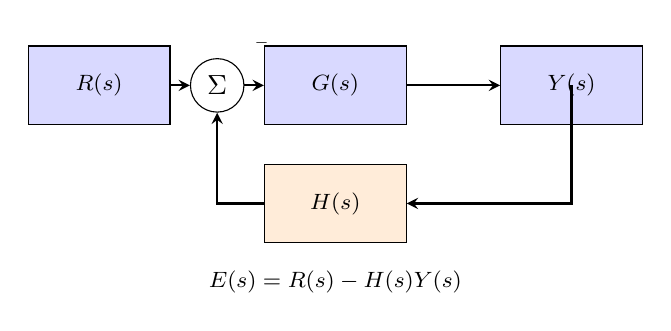
\begin{tikzpicture}[
    ctrlBoxS/.style={rectangle,draw=black,fill=blue!15,minimum width=1.8cm,minimum height=1.0cm,font=\footnotesize},
    ctrlArrowS/.style={->,>=stealth,thick},
]
\node[ctrlBoxS] (ctrlR) at (0,2.0) {$R(s)$};
\node[ctrlBoxS] (ctrlG) at (3,2.0) {$G(s)$};
\node[ctrlBoxS] (ctrlY) at (6,2.0) {$Y(s)$};
\node[ctrlBoxS,fill=orange!15] (ctrlH) at (3,0.5) {$H(s)$};
\node[circle,draw=black,minimum size=0.5cm] (SUM) at (1.5,2.0) {$\Sigma$};
\node at (SUM.north east) [above right=0.1cm, font=\tiny] {$-$};
\draw[ctrlArrowS] (ctrlR.east) -- (SUM.west);
\draw[ctrlArrowS] (SUM.east) -- (ctrlG.west);
\draw[ctrlArrowS] (ctrlG.east) -- (ctrlY.west);
\draw[ctrlArrowS] (6,2.0) -- (6,0.5) -- (ctrlH.east);
\draw[ctrlArrowS] (ctrlH.west) -- (1.5,0.5) -- (SUM.south);
\node[font=\footnotesize] at (3,-0.5) {$E(s)=R(s)-H(s)Y(s)$};
\end{tikzpicture}
\caption{标准单位反馈控制系统框图}
\label{fig:feedback-block}
\end{figure}

\section{传递函数概念}

\subsection{传递函数的定义}

\begin{mydefinition}{传递函数}
对于线性时不变系统，在零初始条件下，传递函数$G(s)$定义为输出量$Y(s)$与输入量$U(s)$的Laplace变换之比：
\[
G(s) = \frac{Y(s)}{U(s)} \;\Big|_{\text{零初始条件}} = \frac{b_m s^m + b_{m-1}s^{m-1} + \cdots + b_1 s + b_0}{a_n s^n + a_{n-1}s^{n-1} + \cdots + a_1 s + a_0}
\]
\end{mydefinition}

传递函数具有以下重要性质：
\begin{itemize}
\item 传递函数仅取决于系统本身的结构和参数，与输入信号形式和初始条件无关。
\item 传递函数是复变量$s$的有理真分式（物理可实现系统满足$m \leq n$）。
\item 传递函数的求解等价于系统微分方程在零初始条件下的Laplace变换。
\item 传递函数不能反映系统内部状态——它只描述输入-输出关系。这也是经典控制理论的根本局限之一。
\end{itemize}

\subsection{极点和零点}

将传递函数写为因式分解形式：
\[
G(s) = K \frac{(s-z_1)(s-z_2)\cdots(s-z_m)}{(s-p_1)(s-p_2)\cdots(s-p_n)}
\]
\begin{itemize}
\item 零点$z_1,z_2,\dots,z_m$——使$G(s)=0$的$s$值。
\item 极点$p_1,p_2,\dots,p_n$——使$G(s) \to \infty$的$s$值。
\item 增益$K$——系统的增益因子，传递函数根轨迹增益。
\end{itemize}

极点和零点在复平面上的分布完全决定了系统的动态特性。

\begin{mydefinition}{特征方程}
系统的特征方程为$A(s)=0$，即$1+G(s)H(s)=0$（闭环）或$A(s)=0$（开环分母）。特征方程的根（即闭环极点）决定了系统自由响应的模态形式。
\end{mydefinition}

例如，若系统具有极点$p = -\sigma \pm j\omega_d$（$\sigma > 0$），则自由响应包含$e^{-\sigma t}\cos(\omega_d t)$形式的振荡衰减模态；若$p = +j\omega$（纯虚极点），则含等幅振荡；若$p = \sigma_j > 0$，则含指数发散模态（不稳定）。

\subsection{极点位置与系统响应关系}

令$s = \sigma + j\omega$。每个极点$p_i = \sigma_i + j\omega_i$对应一个时域模态$e^{p_i t} = e^{\sigma_i t}(\cos\omega_i t + j\sin\omega_i t)$。由此可得：

\begin{itemize}
\item 极点位于左半平面（$\sigma_i < 0$）——响应衰减至零（稳定）。
\item 极点位于虚轴上（$\sigma_i = 0$）——响应等幅振荡（临界稳定）。
\item 极点位于右半平面（$\sigma_i > 0$）——响应发散（不稳定）。
\item 极点实部绝对值越大——衰减越快，暂态过程越短。
\item 极点虚部绝对值越大——振荡频率越高。
\end{itemize}

\section{控制系统的基本要求}

对任何自动控制系统，通常从以下三个方面评价其性能：

\subsection{稳定性}

\begin{mydefinition}{稳定性}
若系统在初始扰动下产生的响应随$t \to \infty$趋于零（即回到原平衡状态），则系统是（渐近）稳定的。数学上等价于所有闭环极点均位于$s$左半平面。
\end{mydefinition}

稳定性是控制系统工作的前提。一个不稳定的系统无法实际运行。线性时不变系统的稳定性完全由其极点位置决定，与输入信号无关。

\subsection{快速性（动态性能）}

快速性描述系统跟踪输入信号的瞬态响应品质，由以下指标衡量：
\begin{itemize}
\item 上升时间$t_r$——响应从稳态值的$10\%$上升至$90\%$（或$0\%$至$100\%$）所需时间。
\item 峰值时间$t_p$——响应达到第一个峰值所需时间。
\item 调节时间$t_s$——响应进入稳态值$\pm(2\%$或$5\%)$误差带后不再逸出的时刻。
\item 超调量$\sigma\%$——最大峰值超出稳态值的百分比。
\end{itemize}

\subsection{准确性（稳态性能）}

准确性即稳态精度，通常用稳态误差$e_{ss} = \lim_{t\to\infty}[r(t) - y(t)]$衡量。

\begin{mydefinition}{系统型别}
设开环传递函数为
\[
G(s)H(s) = \frac{K ( \tau_1 s + 1)(\tau_2 s + 1)\cdots}{s^N (T_1 s + 1)(T_2 s + 1)\cdots}
\]
其中$N$为积分环节的个数（即$s=0$处极点的重数），称系统为$N$型系统。$N=0,1,2$分别对应0型、I型、II型系统。
\end{mydefinition}

型别越高，系统跟踪多项式输入信号的能力越强（稳态误差越小），但稳定性设计也更困难。

\begin{figure}[H]
\centering
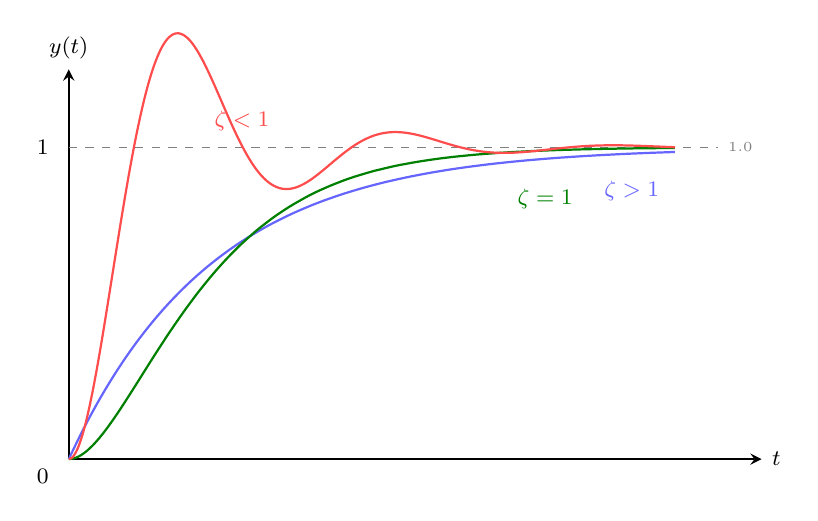
\begin{tikzpicture}[scale=1.1,
    ctrlAxStyle/.style={->,>=stealth,thick},
    ctrlPlot/.style={thick,smooth},
]
% Axes
\draw[ctrlAxStyle] (0,0) -- (8,0) node[right,font=\footnotesize] {$t$};
\draw[ctrlAxStyle] (0,0) -- (0,4.5) node[above,font=\footnotesize] {$y(t)$};
\draw[dashed, gray, thin] (0,3.6) -- (7.5,3.6) node[right, font=\tiny] {1.0};
% Overdamped
\draw[ctrlPlot, blue!60] plot[domain=0:7, samples=100] (\x, {3.6*(1 - exp(-0.6*\x))});
\node[blue!60, font=\footnotesize] at (6.5,3.1) {$\zeta > 1$};
% Critically damped
\draw[ctrlPlot, green!50!black] plot[domain=0:7, samples=100] (\x, {3.6*(1 - (1+1.2*\x)*exp(-1.2*\x))});
\node[green!50!black, font=\footnotesize] at (5.5,3.0) {$\zeta = 1$};
% Underdamped
\draw[ctrlPlot, red!70] plot[domain=0:7, samples=200] (\x, {3.6*(1 - exp(-0.8*\x)*cos(deg(2.5*\x)) - 0.32*exp(-0.8*\x)*sin(deg(2.5*\x)))});
\node[red!70, font=\footnotesize] at (2.0,3.9) {$\zeta < 1$};
% Labels
\node[font=\footnotesize] at (-0.3,3.6) {$1$};
\node[font=\footnotesize] at (-0.3,-0.2) {$0$};
\end{tikzpicture}
\caption{不同阻尼比$\zeta$下的典型二阶系统阶跃响应曲线}
\label{fig:step-responses}
\end{figure}

\subsection*{Python示例：计算并绘制阶跃响应}

\begin{lstlisting}[language=Python]
import numpy as np
import matplotlib.pyplot as plt
from scipy import signal

# 定义二阶系统: G(s) = wn^2 / (s^2 + 2*zeta*wn*s + wn^2)
wn = 1.0  # 自然频率
zeta_values = [0.2, 0.5, 0.707, 1.0, 2.0]

t = np.linspace(0, 20, 1000)
plt.figure(figsize=(10, 6))

for zeta in zeta_values:
    num = [wn**2]
    den = [1, 2*zeta*wn, wn**2]
    sys = signal.TransferFunction(num, den)
    t_out, y = signal.step(sys, T=t)
    plt.plot(t_out, y, linewidth=1.8, label=f'$\\zeta={zeta}$')

plt.xlabel('时间 $t$ (s)')
plt.ylabel('响应 $y(t)$')
plt.title('不同阻尼比下的二阶系统阶跃响应')
plt.legend()
plt.grid(True, alpha=0.3)
plt.axhline(y=1.0, color='gray', linestyle='--', linewidth=0.8)
plt.show()
\end{lstlisting}

\begin{remark}
本章建立了控制理论所需的数学基础。Laplace变换是最核心的工具，它将微分方程转化为代数方程，使传递函数概念成为可能。传递函数的极点和零点分析将在后续各章中贯穿始终。对控制系统稳定性、快速性和准确性的基本要求，构成了整个课程的评价框架。
\end{remark}
